% XCircuit output "control358.tex" for LaTeX input from control358.eps
\def\putbox#1#2#3#4{\makebox[0in][l]{\makebox[#1][l]{}\raisebox{\baselineskip}[0in][0in]{\raisebox{#2}[0in][0in]{\scalebox{#3}{#4}}}}}
\def\rightbox#1{\makebox[0in][r]{#1}}
\def\centbox#1{\makebox[0in]{#1}}
\def\topbox#1{\raisebox{-0.60\baselineskip}[0in][0in]{#1}}
\def\midbox#1{\raisebox{-0.20\baselineskip}[0in][0in]{#1}}
   \scalebox{0.7}{
   \normalsize
   \parbox{3.8125in}{
   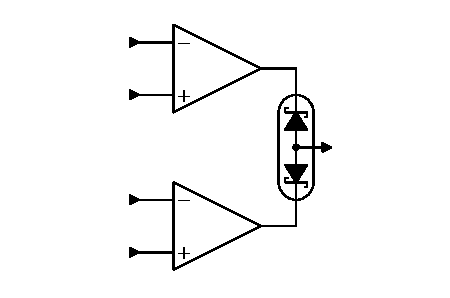
\includegraphics[scale=1.42857]{control358}\\
   % translate x=802 y=312 scale 0.26
   \putbox{1.00in}{2.36in}{1.20}{\rightbox{\midbox{Voltage}}}%
   \putbox{1.00in}{2.19in}{1.20}{\rightbox{\midbox{Feedback}}}%
   \putbox{1.00in}{1.86in}{1.20}{\rightbox{\midbox{Voltage}}}%
   \putbox{1.00in}{1.69in}{1.20}{\rightbox{\midbox{Setpoint}}}%
   \putbox{1.00in}{0.86in}{1.20}{\rightbox{\midbox{Current}}}%
   \putbox{1.00in}{0.36in}{1.20}{\rightbox{\midbox{Current}}}%
   \putbox{1.00in}{0.69in}{1.20}{\rightbox{\midbox{Feedback}}}%
   \putbox{1.00in}{0.19in}{1.20}{\rightbox{\midbox{Setpoint}}}%
   \putbox{3.08in}{1.44in}{1.20}{\midbox{To}}%
   \putbox{3.08in}{1.28in}{1.20}{\midbox{Output}}%
   \putbox{3.08in}{1.11in}{1.20}{\midbox{Amplifier}}%
   } % close 'parbox'
   } % close 'scalebox'
   \vspace{-\baselineskip} % this is not necessary, but looks better
